\documentclass[11pt]{article}
\usepackage{geometry,marginnote} % Pour passer au format A4
\geometry{hmargin=1cm, vmargin=1.5cm} % 

% Page et encodage
\usepackage[T1]{fontenc} % Use 8-bit encoding that has 256 glyphs
\usepackage[english,french]{babel} % Français et anglais
\usepackage[utf8]{inputenc} 

\usepackage{lmodern}
\usepackage[np]{numprint}
\setlength\parindent{0pt}

% Graphiques
\usepackage{graphicx,float,grffile}
\usepackage{tikz,pst-eucl,pst-plot,pstricks,pst-node,pstricks-add,pst-fun,pgfplots} 

% Maths et divers
\usepackage{amsmath,amsfonts,amssymb,amsthm,verbatim,scratch3}
\usepackage{multicol,enumitem,url,eurosym,gensymb,tabularx}

\DeclareUnicodeCharacter{20AC}{\euro}



% Sections
\usepackage{sectsty} % Allows customizing section commands
\allsectionsfont{\centering \normalfont\scshape}

% Tête et pied de page
\usepackage{fancyhdr} \pagestyle{fancy} \fancyhead{} \fancyfoot{}

%\fancyfoot[L]{Collège Faubert}
%\fancyfoot[C]{\thepage / 6}
%\fancyfoot[R]{Série Générale}

\renewcommand{\headrulewidth}{0pt} % Remove header underlines
%\renewcommand{\footrulewidth}{0pt} % Remove footer underlines

\newcommand{\horrule}[1]{\rule{\linewidth}{#1}} % Create horizontal rule command with 1 argument of height

\newcommand{\Pointilles}[1][3]{%
  \multido{}{#1}{\makebox[\linewidth]{\dotfill}\\[\parskip]
}}

\newtheorem{Definition}{Définition}

\usepackage{siunitx}
\sisetup{
    detect-all,
    output-decimal-marker={,},
    group-minimum-digits = 3,
    group-separator={~},
    number-unit-separator={~},
    inter-unit-product={~}
}

\setlength{\columnseprule}{1pt}


\begin{document}

\textbf{Nom, Prénom :} \hspace{8cm} \textbf{Classe :} \hspace{3cm} \textbf{Date :}\\
\vspace{-0.8cm}
\begin{center}
  \textit{Si nous faisions tout ce dont nous sommes capables, nous nous surprendrions vraiment.}  - \textbf{Thomas Edison}
\end{center}
\vspace{-0.8cm}

\subsection*{Définitions}
  \begin{enumerate}
    \item[1.] Tableau de proportionnalité : \dotfill \\
    \Pointilles[2]
    \item[2.] La représentation graphique d'une situation de proportionnalité est \dotfill \\
    \Pointilles[1]
  \end{enumerate}

\subsection*{Exercice 1 - Calculer - (Les tableaux sont proportionnels)}

\begin{multicols}{4}\noindent
  \begin{center}
    \begin{tabular}{|c|c|}
      \hline
      1 & 32\\  \hline
      14,5 & $\phantom{azertyuiop}$\\  \hline
    \end{tabular}
  \end{center}
  \Pointilles[2]
  \begin{center}
    \begin{tabular}{|c|c|}
      \hline
      12 & $\phantom{azertyuiop}$\\  \hline
      1,5 & 24\\  \hline
    \end{tabular}
  \end{center}
  \Pointilles[2]
  \begin{center}
    \begin{tabular}{|c|c|}
      \hline
      $\phantom{azertyuiop}$  & 24\\  \hline
      8 & 68\\  \hline
    \end{tabular}
  \end{center}
  \Pointilles[2]
  \begin{center}
    \begin{tabular}{|c|c|}
      \hline
      12 & 46\\  \hline
      $\phantom{azertyuiop}$ & 24\\  \hline
    \end{tabular}
  \end{center}
  \Pointilles[2]
\end{multicols}

\begin{center}
  \begin{tabular}{|c|c|c|c|c|c|}
    \hline
   3 &  3,1                   &                  45000 &  \phantom{100 000 000} &  \phantom{100 000 000} &                     9\\ \hline
   7 &  \phantom{100 000 000} &  \phantom{100 000 000} &                   7400 &                    0,4 &  \phantom{100 000 000}\\ \hline     
  \end{tabular}
\end{center}
\Pointilles[4]


\subsection*{Exercice 2 - Démontrer si le tableau est proportionnel}

\begin{multicols}{2}
  \begin{center}
    \begin{tabular}{|c|c|c|}
      \hline
      24 & 96 & 212 \\  \hline
      2 & 8 & 26\\  \hline
    \end{tabular}
  \end{center}
  \begin{center}
    \begin{tabular}{|c|c|c|}
      \hline
      12 & 18 & 6 \\  \hline
      30 & 45 & 15\\  \hline
    \end{tabular}
  \end{center}
\end{multicols}

\Pointilles[6]


\subsection*{Problèmes}

\begin{minipage}[t]{0.25\textwidth}
  \begin{figure}[H]
    \centering
    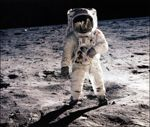
\includegraphics[width=100px]{4x3-proportionnalite/ex1.jpg}
  \end{figure}
\end{minipage}
\begin{minipage}[t]{0.75\textwidth}
\textbf{1.} La fusée Starship de SpaceX se déplace à la vitesse de 12 000km/h. 

\begin{enumerate}
  \item[1.] Combien de temps peut-elle mettre pour rejoindre la lune située à 384 400km ? 
  \item[2.] Quelle est la distance parcourue en 2h30min ? 
\end{enumerate}

\Pointilles[2]
\end{minipage}

\Pointilles[6]

\newpage

\begin{minipage}[t]{0.25\textwidth}
  \begin{figure}[H]
    \centering
    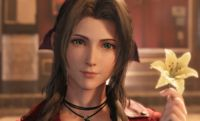
\includegraphics[width=100px]{4x3-proportionnalite/ex2.jpg}
  \end{figure}
\end{minipage}
\begin{minipage}[t]{0.75\textwidth}
\textbf{2.} Il est possible de convertir des euros (€) en gils (G) en suivant la règle : 5€ = 13G.

\begin{enumerate}
  \item[1.] Tifa souhaite acheter une jolie cape. Elle coûte 225G. Quel est son prix en euros ? 
  \item[2.] Aerith souhaite plutôt acheter un beau gilet rose. Elle possède 53€. Quel prix maximal peut-elle mettre en gils?
\end{enumerate}

\Pointilles[1]
\end{minipage}

\Pointilles[7]

\begin{minipage}[t]{0.25\textwidth}
  \begin{figure}[H]
    \centering
    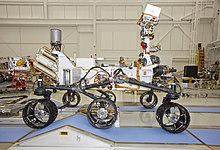
\includegraphics[width=100px]{4x3-proportionnalite/ex3.jpg}
  \end{figure}
\end{minipage}
\begin{minipage}[t]{0.75\textwidth}
\textbf{3.} Le rover Curiosity est actuellement sur Mars. Il est composé principalement de titane. On a utilisé des tubes de 5m qui ont une masse de 32.4kg. 

\begin{enumerate}
  \item[1.] Quelle est la longueur d'un tube de 100kg ?
  \item[2.] Quelle est la masse d'un tube de 46.7m ? 
\end{enumerate}

\Pointilles[3]
\end{minipage}

\Pointilles[5]

\begin{minipage}[t]{0.25\textwidth}
  \begin{figure}[H]
    \centering
    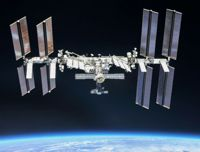
\includegraphics[width=100px]{4x3-proportionnalite/ex4.jpg}
  \end{figure}
\end{minipage}
\begin{minipage}[t]{0.75\textwidth}
\textbf{4.} Pour respirer normalement dans l'ISS, les astronautes doivent faire un mélange gazeux. Il faut mélanger 7L d'oxygène et 30L d'azote.  

Comment obtenir 200L d'air respirable ?

\Pointilles[5]
\end{minipage}

\Pointilles[5]

\begin{minipage}[t]{0.25\textwidth}
  \begin{figure}[H]
    \centering
    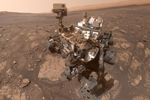
\includegraphics[width=100px]{4x3-proportionnalite/ex5.jpg}
  \end{figure}
\end{minipage}
\begin{minipage}[t]{0.75\textwidth}
\textbf{5.} Un volcan rentre en irruption en antarctique. La température de la lave à la sortie du cratère est de $840 \degree C$. La lave est projetée sur de la banquise qui a une température de $-27\degree C$.

Quelle est la différence de température ?

\Pointilles[3]
\end{minipage}

\Pointilles[2]

\newpage


\textbf{Nom, Prénom :} \hspace{8cm} \textbf{Classe :} \hspace{3cm} \textbf{Date :}\\
\vspace{-0.8cm}
\begin{center}
  \textit{Si nous faisions tout ce dont nous sommes capables, nous nous surprendrions vraiment.}  - \textbf{Thomas Edison}
\end{center}
\vspace{-0.8cm}

\subsection*{Définitions}
  \begin{enumerate}
    \item[1.] Tableau de proportionnalité : \dotfill \\
    \Pointilles[2]
    \item[2.] La représentation graphique d'une situation de proportionnalité est \dotfill \\
    \Pointilles[1]
  \end{enumerate}

\subsection*{Exercice 1 - Calculer - (Les tableaux sont proportionnels)}

\begin{multicols}{4}\noindent
  \begin{center}
    \begin{tabular}{|c|c|}
      \hline
      1 & 22\\  \hline
      12,5 & $\phantom{azertyuiop}$\\  \hline
    \end{tabular}
  \end{center}
  \Pointilles[2]
  \begin{center}
    \begin{tabular}{|c|c|}
      \hline
      14 & $\phantom{azertyuiop}$\\  \hline
      1,4 & 21\\  \hline
    \end{tabular}
  \end{center}
  \Pointilles[2]
  \begin{center}
    \begin{tabular}{|c|c|}
      \hline
      $\phantom{azertyuiop}$  & 26\\  \hline
      9 & 48\\  \hline
    \end{tabular}
  \end{center}
  \Pointilles[2]
  \begin{center}
    \begin{tabular}{|c|c|}
      \hline
      11 & 33\\  \hline
      $\phantom{azertyuiop}$ & 22\\  \hline
    \end{tabular}
  \end{center}
  \Pointilles[2]
\end{multicols}

\begin{center}
  \begin{tabular}{|c|c|c|c|c|c|}
    \hline
   5 &  5,1                   &                  65000 &  \phantom{100 000 000} &  \phantom{100 000 000} &                     15\\ \hline
   9 &  \phantom{100 000 000} &  \phantom{100 000 000} &                   8400 &                    0,3 &  \phantom{100 000 000}\\ \hline     
  \end{tabular}
\end{center}
\Pointilles[4]


\subsection*{Exercice 2 - Démontrer si le tableau est proportionnel}

\begin{multicols}{2}
  \begin{center}
    \begin{tabular}{|c|c|c|}
      \hline
      22 & 132 & 286 \\  \hline
      2 & 11 & 26\\  \hline
    \end{tabular}
  \end{center}
  \begin{center}
    \begin{tabular}{|c|c|c|}
      \hline
      8 & 18 & 6 \\  \hline
      32 & 72 & 25\\  \hline
    \end{tabular}
  \end{center}
\end{multicols}

\Pointilles[6]


\subsection*{Problèmes}

\begin{minipage}[t]{0.25\textwidth}
  \begin{figure}[H]
    \centering
    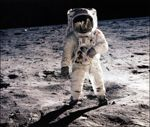
\includegraphics[width=100px]{4x3-proportionnalite/ex1.jpg}
  \end{figure}
\end{minipage}
\begin{minipage}[t]{0.75\textwidth}
\textbf{1.} La fusée Starship de SpaceX se déplace à la vitesse de 13 000km/h. 

\begin{enumerate}
  \item[1.] Quelle est la distance parcourue en 5h30min ? 
  \item[2.] Combien de temps peut-elle mettre pour rejoindre la lune située à 289 400km ? 
\end{enumerate}

\Pointilles[2]
\end{minipage}

\Pointilles[6]

\newpage

\begin{minipage}[t]{0.25\textwidth}
  \begin{figure}[H]
    \centering
    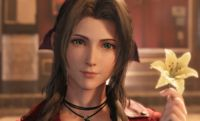
\includegraphics[width=100px]{4x3-proportionnalite/ex2.jpg}
  \end{figure}
\end{minipage}
\begin{minipage}[t]{0.75\textwidth}
\textbf{2.} Il est possible de convertir des euros (€) en gils (G) en suivant la règle : 5€ = 17G.

\begin{enumerate}
  \item[1.] Tifa souhaite acheter une jolie cape. Elle coûte 325G. Quel est son prix en euros ? 
  \item[2.] Aerith souhaite plutôt acheter un beau gilet rose. Elle possède 53€. Quel prix maximal peut-elle mettre en gils?
\end{enumerate}

\Pointilles[1]
\end{minipage}

\Pointilles[7]

\begin{minipage}[t]{0.25\textwidth}
  \begin{figure}[H]
    \centering
    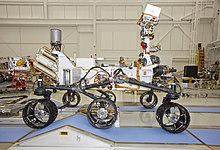
\includegraphics[width=100px]{4x3-proportionnalite/ex3.jpg}
  \end{figure}
\end{minipage}
\begin{minipage}[t]{0.75\textwidth}
\textbf{3.} Le rover Curiosity est actuellement sur Mars. Il est composé principalement de titane. On a utilisé des tubes de 5m qui ont une masse de 41.3kg. 

\begin{enumerate}
  \item[1.] Quelle est la longueur d'un tube de 100kg ?
  \item[2.] Quelle est la masse d'un tube de 46.7m ? 
\end{enumerate}

\Pointilles[3]
\end{minipage}

\Pointilles[5]

\begin{minipage}[t]{0.25\textwidth}
  \begin{figure}[H]
    \centering
    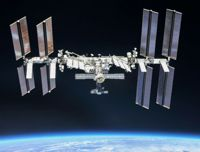
\includegraphics[width=100px]{4x3-proportionnalite/ex4.jpg}
  \end{figure}
\end{minipage}
\begin{minipage}[t]{0.75\textwidth}
\textbf{4.} Pour respirer normalement dans l'ISS, les astronautes doivent faire un mélange gazeux. Il faut mélanger 6L d'oxygène et 31L d'azote.  

Comment obtenir 300L d'air respirable ?

\Pointilles[5]
\end{minipage}

\Pointilles[5]

\begin{minipage}[t]{0.25\textwidth}
  \begin{figure}[H]
    \centering
    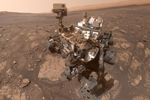
\includegraphics[width=100px]{4x3-proportionnalite/ex5.jpg}
  \end{figure}
\end{minipage}
\begin{minipage}[t]{0.75\textwidth}
\textbf{5.} Un volcan rentre en irruption en antarctique. La température de la lave à la sortie du cratère est de $860 \degree C$. La lave est projetée sur de la banquise qui a une température de $-29\degree C$.

Quelle est la différence de température ?

\Pointilles[3]
\end{minipage}

\Pointilles[2]
\end{document}